\section{El modelo Transformer}

A finales del año 2017 se presentó un nuevo modelo que vino a revolucionar el área de Procesamiento
de Lenguaje Natural, El Transformer \cite{Vaswani}. Una de sus principales características es la
capacidad de procesar la información de alguna secuencia de forma paralela, caso contrario a las
Redes Neuronales Recurrentes, donde la información se procesa recurrentemente. Gracias a ello,
la capacidad de \textit{recuerdo} no se ve afectado por el problema de \textit{El desvanecimiento
del Gradiente} específicamente cuando el problema es trabajar con secuencias  bastante largas.

\textit{El Transformer} puede ser visto como otro modelo \textit{seq2seq} (Secuencia a Secuencia)
\ref{fig:trans_seq2sqe}, formado en por dos etapas, la primera encargada de codificar la información de entrada
y la segunda de decodificarla, pero la su principal característica es que aplica el mecanismos de
\textit{Self-Attention} para capturar las dependencias globales entre la entrada y la salida. Dada
una secuencia de entrada $X = (x_1, x_2, \dots, x_n )$ con $n$ como el tamaño de la secuencia,
el codificador produce una representación intermedia
$Z = (z_1, z_2, \dots, z_n)$ al igual que los modelos \textit{seq2seq}. El decodificador usa la
secuencia $Z$ para generar la secuencia de salida
$Y = (y_1, y_2, \dots, y_m)$ uno a la vez (en modo inferencia), con $m$ como el tamaño de la
secuencia de salida. Nótese, que el generar una salida a la vez el decodificador tiene que ser auto-regresivo.
Usa la salida anterior $y_{i-1}$ como entrada adicional para generar la siguiente salida $y_i$. Por
ello, durante entrenamiento el modelo es alimentado con entradas y salidas desfasadas en un tiempo.

\begin{figure}[ht!]
    \centering
    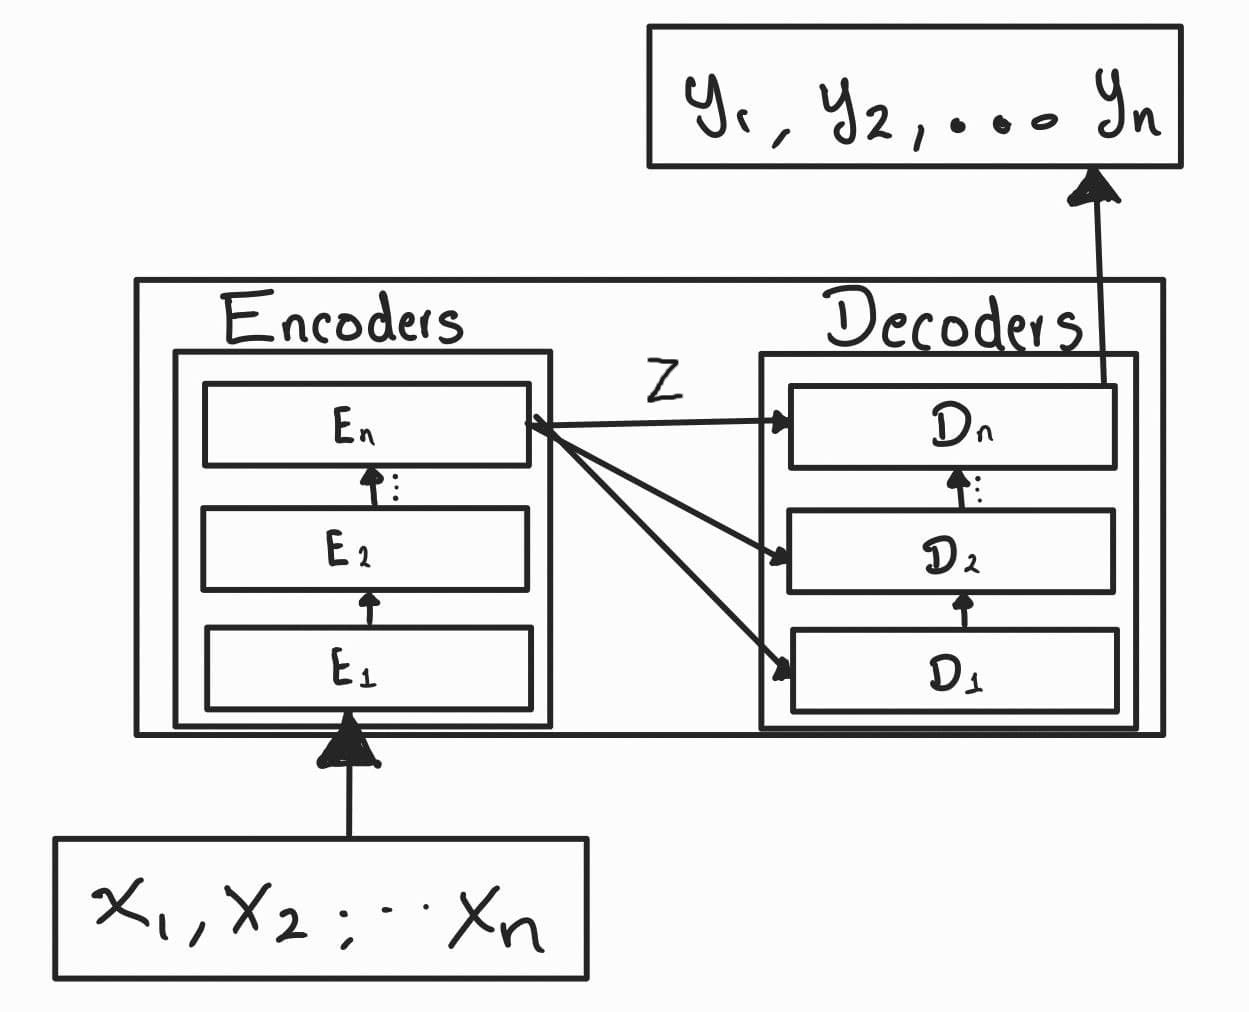
\includegraphics[width=0.4 \textwidth]{Chapters/1. Transformer/Figures/transformer/t_seq2seq.jpg}
    \caption{Modelo Transformer generalizado como modelo Secuencia a Secuencia}
    \label{fig:trans_seq2sqe}
\end{figure}

Poner ejemplo de Transformer en con la figura de arriba en tiempo de entrenamiento e inferencia aquí.

\subsection{El Codificador y Decodificador}

El \textit{Modelo Transformer} está formado por multiples codificadores  y decodificadores apilados e inter-conectados,
Como observamos en la figura \ref{fig:trans_seq2sqe}. El codificador consta de dos partes,
la primera de ellas aplica \textit{Self-Attention} múltiples veces sobre la misma entrada
(\textit{Multi-HeadSelf Attention}) y la segunda capa representada solo por una red
\textit{Feed-Forward} cuya entrada es la salida de la capa anterior.
Véase la figura \ref{fig:trans_encoder}.


\begin{figure}[ht!]
\centering
    \begin{minipage}{.4\textwidth}
        \centering
        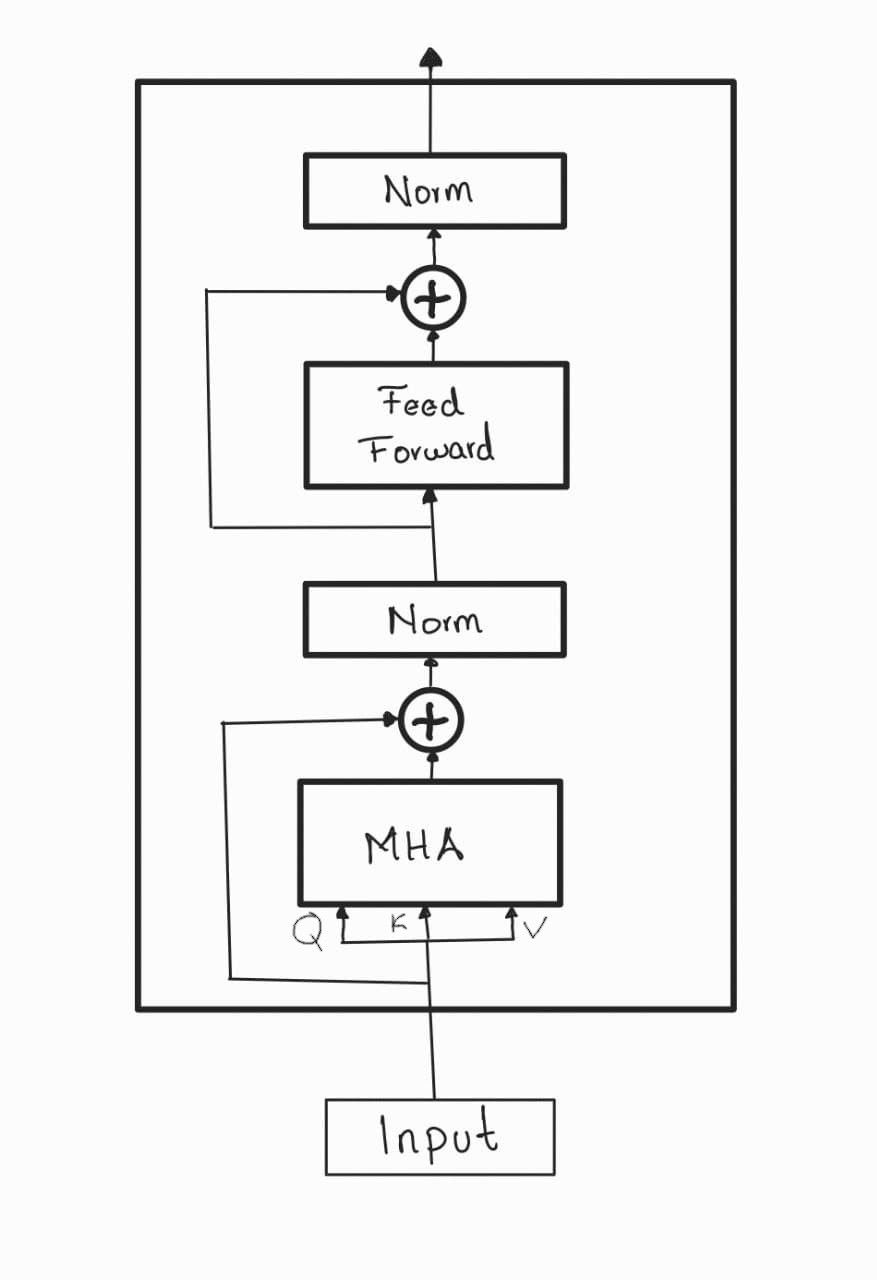
\includegraphics[width=0.7 \textwidth]{Chapters/1. Transformer/Figures/transformer/encoder.jpg}
    \end{minipage}
    \begin{minipage}{.5\textwidth}
        \begin{equation*}
            \begin{split}
                mha = MHA(X)\\
                norm = Norm( mha + X)\\
                f = FeedForward(norm)\\
                Encoder(X) = Norm(f + norm)
            \end{split}
            \label{eq:trans_enc}
        \end{equation*}
    \end{minipage}
    \caption{Etapa Codificadora del Modelo Transformer}.
    \label{fig:trans_encoder}
\end{figure}


El decodificador tiene una estructura similar al codificador con una etapa adicional al inicio
de \textit{Multi-Head Attention}.
